\documentclass[11pt]{article}
\usepackage{times,latexsym,amsmath,amssymb,amsfonts,bm,mathtools}
\usepackage{array, marginnote, paralist, booktabs, multirow, url, natbib}
\usepackage{graphicx, epstopdf, rotating, color, subfig, adjustbox}
\usepackage[linesnumbered,lined,boxed,commentsnumbered]{algorithm2e}
\usepackage[margin=1in]{geometry}
\usepackage[margin=1in]{caption}
\usepackage{relsize}
\usepackage{amsthm}

\SetKwInOut{Parameter}{parameter}
\renewcommand{\familydefault}{ptm}
\setlength{\parindent}{0cm}
\setlength{\parskip}{1em}%
\newcommand{\HRule}{\rule{\linewidth}{0.5mm}}
\newcommand{\mean}{\text{mean}}
\newcommand{\sd}{\text{sd}}
\newcommand{\median}{\text{median}}
\newcommand{\IQR}{\text{IQR}}
\newcommand{\MAD}{\text{MAD}}
\newcommand{\dist}{\text{dist}}
\newcommand{\diag}{\text{diag}}
\newcommand{\nn}{\text{nn}}
\newcommand{\nnd}{\text{nnd}}
%\DeclareMathOperator*{\argmax}{arg\,max}
%\DeclareMathOperator*{\argmin}{arg\,min}
\newcommand{\argmin}{\mathop{\text{argmin}}}
\newcommand{\argmax}{\mathop{\text{argmax}}}
\newcolumntype{d}[1]{D{.}{.}{#1}}  % define "d" column type

\newcommand{\density}{\text{density}}
\newcommand{\AUC}{\text{AUC}}
\newcommand{\margincomment}[1]{\marginpar{\footnotesize{#1}}}
\newtheorem{theorem}{Theorem}[section]
\newtheorem{definition}[theorem]{Definition}
\newtheorem{proposition}[theorem]{Proposition}

\graphicspath{{./Graphics/}}

\newcommand{\chk}{$\checkmark$}
\newcolumntype{R}[2]{%
    >{\adjustbox{angle=#1,lap=\width-(#2)}\bgroup}%
    l%
    <{\egroup}%
}
\newcommand*\rot{\multicolumn{1}{R{90}{1em}}}% no optional argument here, please!

% =======================================================================
\begin{document}
% =======================================================================
\title{Outlier Components: A basis suitable for outlier detection}
\author{Sevvandi Kandanaarachchi, Rob J. Hyndman}
\maketitle
\abstract{FOR LATER}

% =======================================================================
\section{Introduction}
% =======================================================================
FOR LATER!

% =======================================================================
\section{Related work}
% =======================================================================
FOR LATER!

% =======================================================================
\section{Mathematical Framework}\label{sec:MathFrame}
% =======================================================================
Let $X_{N \times p}$ be a matrix denoting a dataset of $N$ observations and $p$ attributes. Let us denote the  $i^{\text{th}}$ observation in $X$ by $\bm{x}_i$. The  distance between points $\bm{x}_i$ and $\bm{x}_j$  can be written as 
\begin{equation}\label{eq:secMF1}
\dist(\bm{x}_i, \bm{x}_j)^2 = \left( \bm{x}_i - \bm{x}_j \right)^T S \left( \bm{x}_i - \bm{x}_j \right) \, , 
\end{equation}
where $S$ is a symmetric positive definite matrix.  In addition when $S$ is diagonal, i,e, $S = \diag(s_1, s_2, \ldots s_p)$ we obtain
\begin{equation}\label{eq:secMF2}
    \dist(\bm{x}_i, \bm{x}_j)^2 = \left\langle \eta\, ,  \left( \bm{x}_i - \bm{x}_j \right)^2 \right\rangle\, 
\end{equation}
where $\left\langle \cdot\, , \cdot \right\rangle$ denotes the standard inner product in $\mathbb{R}^p$,   $\eta = \left(s_1, s_2, \ldots s_p\right)^T$, and with some abuse of notation $\left( \bm{x}_i - \bm{x}_j \right)^2$ denotes the element wise difference of $\left( \bm{x}_i - \bm{x}_j \right)$ squared. As $S$ is symmetric and positive definite  it is diagonalizable, thus giving us motivation for considering a diagonal $S$. 

\subsection{The $Y$ space}\label{sec:MathFrame1}
Let  $\bm{y}_{ij} = \left( \left( x_{i1} - x_{j1} \right)^2, \left( x_{i2} - x_{j2} \right)^2, \ldots,  \,  \left( x_{ip} - x_{jp} \right)^2  \right)\, . $ Substituting in equation~\eqref{eq:secMF2} gives
\begin{equation}\label{eq:secMF3}
    \dist(\bm{x}_i, \bm{x}_j)^2 = \left\langle \eta\, ,  \bm{y}_{ij} \right\rangle\, \, .
\end{equation}
As such, by finding the appropriate $\eta$ of unit length,  we can maximize the distance between $\bm{x}_i$ and $\bm{x}_j$.  This brings us to the question of which $\bm{x}_i$ and $\bm{x}_j$ needs to be chosen to maximize the distance between them. If we use knn distances as a guiding principle, we are interested in the $k$ nearest neighbours of a given point. Consequently, we can choose $\bm{x}_i$ and $\bm{x}_j$ that share a common neighbourhood. Also we note that if we were to calculate $\bm{y}_{ij}$ for all pairs, it would be computationally expensive as there are $N(N+1)/2$ pairs. In addition, this would give us pairwise distances between points that we are not interested in, such as points on the boundary of the point cloud, that are opposite each other. Finding  $\eta$ that maximizes the distances between such points is not conducive to outlier detection, because a large distance between such polar-opposite points does not mean that either of those points are outliers. As such, we select the  $\bm{x}_i$ and $\bm{x}_j$ pairs that we want to include in our $Y$ space. \\

For each point $\bm{x}_i$ we compute $\bm{y}_{ij}$ arising from a set a nearest neighbours. From \cite{kandanaarachchi2018normalization} we know that nearest neighbours depend on the normalization technique. As a result, we choose two normalization techniques for pre-processing the data; Min-Max and Median-IQR. Min-Max normalization scales each column to values between $0$ and $1$, with the minimum mapped to $0$ and the maximum mapped to $1$.  Median-IQR scales each column to median $0$ and IQR $1$. Let $X_1$ denote the normalized data using  Min-Max and $X_2$ using Median-IQR. For each normalization technique we choose a set of nearest neighbours from $k_1$ to $k_2$, that is for any point we choose the $k_1^{\text{th}}$ nearest neighbour to  $k_2^{\text{th}}$ nearest neighbour. Here $k_1$ and $k_2$ are parameters and one can choose $k_1 =0$. \\

Next for each point we find the union of nearest neighbours computed using the two normalization techniques. For example for a given point $\bm{x}_i$ if Min-Max gave rise to the nearest neighbours $\{\bm{x}_2, \bm{x}_5, \bm{x}_9 \}$ and Median-IQR   $\{\bm{x}_5, \bm{x}_4, \bm{x}_7 \}$, then we consider the union of these two sets as the set of nearest neighbours of $\bm{x}_i$. Using the nearest neighbours we construct a list of pairs denoted by $T$. Continuing the same example the pairs $(\bm{x}_i, \bm{x}_2), \,  (\bm{x}_i, \bm{x}_5), \, (\bm{x}_i, \bm{x}_4), \, \ldots $ and so on will be in $T$. \\

For each pair in $T$, we compute $\bm{y}_{ij}$ as in equation~\eqref{eq:secMF2} on the normalized space $X_1$ or $X_2$, depending on user preference. Now we have the initial $Y$ space; a set of $M$ points in $\mathbb{R}^{p+}$. As the pairs of points that give rise to the initial $Y$ space are contained in $T$, we can refer to $Y = \{ \bm{y}_l \}_{l=1}^M$, where each $\bm{y}_l = \bm{y}_{i_{(l)}, j_{(l)} }$, i.e. $l$ is the row number in the matrix $Y$ and each $\bm{y}_l$ comes from the $l^{\text{th}}$ pair in $T$. \\

We are interested in neighbouring distances that are relatively large. The Euclidean distance squared between two points in the $X_1$ or $X_2$ space  can be written as $\sum_{m=1}^p y_{lm}$ for the appropriate $l$. In order to consider only points with relatively large distances, we remove points $\bm{y}_l$ that contribute to distances below a certain percentile, i.e. we remove points $\bm{y}_l$ such that  $\sum_{m=1}^p y_{lm} < Q$ where $Q$ is the $q^{\text{th}}$ percentile of $ \left \{\sum_{m=1}^p y_{lm} \right \}_{l=1}^M$. We remove the associated pairs from $T$ as well. This constitutes the $Y$ space. \\

The main advantage of the $Y$ space is that it makes distance computation  between two points in the $X$ space a linear function. This makes maximizing distances between points a much easier task. 
Algorithm~\ref{algo:YSpace} summarizes the construction of the $Y$ space. 

%The user-defined parameters for the construction of the $Y$ space are $k_1, k_2$ and $q$, with default values of 

\DontPrintSemicolon
\begin{algorithm}\fontsize{9}{10}\selectfont
	\SetKwInOut{Input}{input~~~}
	\SetKwInOut{Output}{output}
	\Input{~$X$, $k_1, k_2 \in \mathbb{Z}^+$ and $q \in (0, 1)$.}
	\Output{~The space $Y$ consisting of all $y_{ij}$ pairs and the associated indices $i$ and $j$.}
	Normalize $X$ using Min-Max normalization. Let us call this space $X_1$.  \\
	Find $k_1$ to $k_2$ nearest neighbours for each point in  $X_1$. \\
	Next normalize $X$ using Median-IQR normalization. Let us call this space $X_2$.  \\
	Find $k_1$ to $k_2$ nearest neighbours for each point in  $X_2$. \\
	Then for each point collate all unique neighbours using both Min-Max and Median-IQR normalization methods.   \\
	Let $T = $ the set of $i$ and $j$ indices, corresponding to the pairs of points in $X$. \\
	For all these pairs, compute $\bm{y}_{ij}$ as in equation~\eqref{eq:secMF3} using $X_1$ space. Let $Y =\left\{ \bm{y}_{1} =\bm{y}_{i_{(1)},j_{(1)}} , \bm{y}_{2} =\bm{y}_{i_{(2)},j_{(2)}}, \ldots, \bm{y}_{M} =\bm{y}_{i_{(M)},j_{(M)}} \right\}$, where $\left( i_{(1)},j_{(1)} \right)$ is the first $(i, j)$ pair. Consequently $Y$ is an $M\times p$ matrix, with the $l^{\text{th}}$ row denoted by $\bm{y}_l$.\\
	Find the $q^{\text{th}}$ percentile of $ \left\{\sum_{m=1}^p \bm{y}_{lm}\right\}$. The quantity $\sum_{m=1}^p \bm{y}_{lm}$ is the distance between points $\bm{x}_{i_{(l)}}$ and $\bm{x}_{j_{(l)}}$ in  $X_1$  space. \\
	Remove points $\bm{y}_l$ which are less than the  $q^{\text{th}}$ percentile of  $ \sum_{m=1}^p \bm{y}_{lm} $. \\
	Remove the associated pairs of $(i, j)$ from $T$.
	\caption{\itshape Construction of the $Y$ space}
	\label{algo:YSpace}
\end{algorithm}

\begin{figure}[!t]
	\centering
	\subfloat[][]{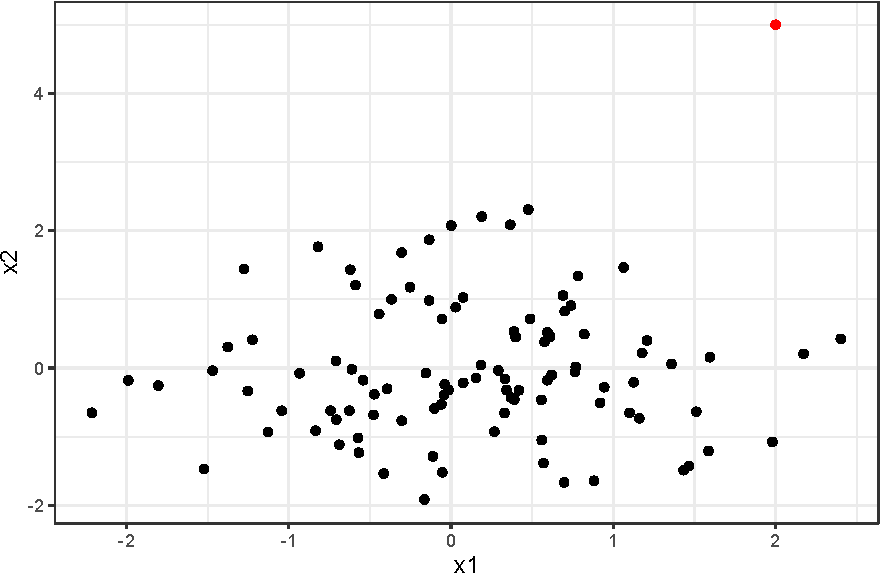
\includegraphics[scale=0.5]{X_space.pdf}\label{fig:XandY1}}
	\subfloat[][]{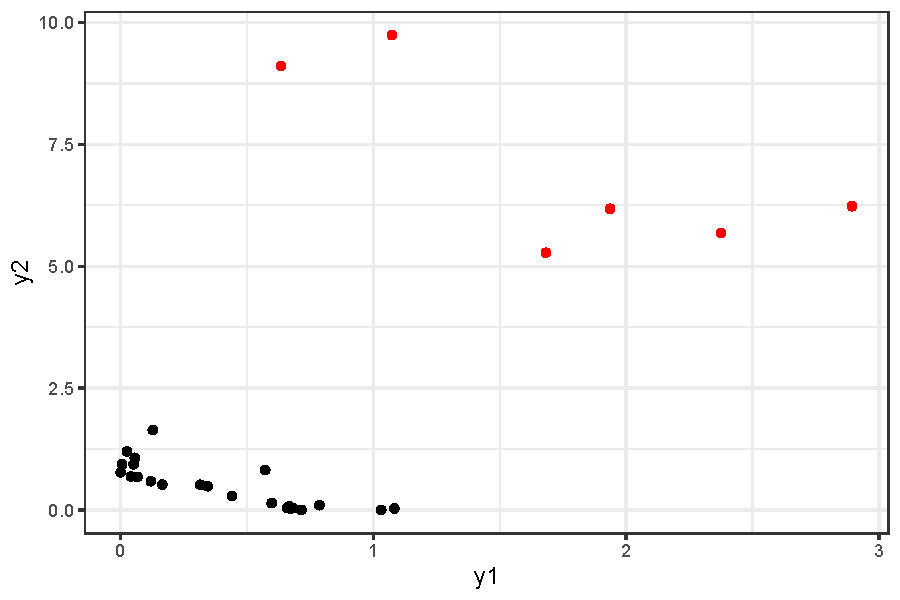
\includegraphics[scale=0.5]{Y_space.pdf}\label{fig:XandY2}}
	\caption{The $X$ and $Y$ spaces. The $X$ space in (a) and the associated $Y$ space in (b) with $q = 0.95$. The red coloured point in the $X$ space gives rise to 6   points, which are coloured in red in the $Y$ space.}
	\label{fig:XandY}
\end{figure} 

%% Explanation of fig:XandY
Figure~\ref{fig:XandY} illustrates  the $X$ and $Y$ spaces for which the $X$ space is a 2 dimensional normal distribution of 100 points with a single outlier depicted in red. We see that the $Y$ space consists of a lesser number of points, of which 6 points are contributed by the outlier. This is because $k_1$ to $k_2$ neighbours are considered in the construction of the $Y$ space and the  points $\bm{y}_k$ with relatively small distances $\left(\sum_i y_{ki} \leq Q\right)$ are removed. Thus, the effect of outliers are magnified in the $Y$ space. \\

Before turning to maximising distances, we summarise  key features of the $Y$ space below:
\begin{enumerate}
    \item $Y = \{\bm{y}_l \}_{l=1}^M$, where $\bm{y}_l \in \mathbb{R}^{p+}$.
    \item Each $\bm{y}_l \in Y$ is constructed from two points $\bm{x}_i$ and $\bm{x}_j$ in $X$ with $T(l) = (i,j)$, where $T$ is a matrix consisting of the list of pairs in $X$ that are used to construct $Y$. In addition $\bm{x}_i$ and $\bm{x}_j$ are $k$-nearest neighbours for some $k \in \{k_1, \ldots, k_2\}$.
    \item For $i,j,l$ as in above,  $\bm{y}_l = \left(\bm{x}_i - \bm{x}_j \right)^2$, where with some abuse of notation $\left(\bm{x}_i - \bm{x}_j \right)^2$ denotes the element-wise difference squares. 
    \item The $Y$ space contains points $\bm{y}_l$ with relatively high $\sum_{m=1}^p y_{lm}$.  
\end{enumerate}

\subsection{Maximising the distance between points}\label{sec:MathFrame2}
The $Y$ space has points $\bm{y}_l$ that correspond to neighbouring points $\bm{x}_i$ and $\bm{x}_j$ in $X$, which have relatively high $k$ nearest neighbour distances. From equation~\eqref{eq:secMF3} we obtain
\begin{equation} \label{eq:secMF4}
    \sum_{(i,j) \in T}\dist(\bm{x}_i, \bm{x}_j)^2 = \sum_{l}\left\langle \eta\, ,  \bm{y}_{l} \right\rangle\, \, .
\end{equation}
Thus  the total distance squared for relatively high nearest neighbour distances $ \sum_{(i,j) \in T}\dist(\bm{x}_i, \bm{x}_j)^2$  can be maximised by finding the appropriate $\eta$ which maximises $\sum_{l}\left\langle \eta\, ,  \bm{y}_{l} \right\rangle$. However, by choosing $\eta_1 = c \eta_0 $, with $c >1$ will automatically increase the value of $\sum_{l}\left\langle \eta\, ,  \bm{y}_{l} \right\rangle$ by $c$. Thus, we restrict $\eta$ such that $\left \lVert \eta \right\rVert = 1$.  We now state our optimisation problem as
\begin{align} \label{eq:secMF5}
     \max_\eta & \sum_{l}\left\langle \eta\, ,  \bm{y}_{l} \right\rangle \, , \\ 
    \left \lVert \eta \right\rVert^2  & = 1 \notag \, .
\end{align}
Solving this using Lagrange Multipliers we obtain $\nabla f  = \lambda \nabla g$, with 
\begin{align}\label{eq:secMF6}
    f(\eta) & = \sum_{l}\left\langle \eta\, ,  \bm{y}_{l} \right\rangle  \, , \text{and} \\
    g(\eta)  & = \left \lVert \eta \right\rVert^2  - 1 = 0 \, . \notag
\end{align}
As $\nabla f = \left( \frac{\partial f}{\partial \eta_1},  \frac{\partial f}{\partial \eta_2},  \cdots, \frac{\partial f}{\partial \eta_p} \right)$ we compute
\begin{align}\label{eq:secMF7}
\frac{\partial f}{\partial \eta_j} & =  \frac{\partial }{\partial \eta_j}\sum_{l}\left\langle \eta\, ,  \bm{y}_{l} \right\rangle \, ,  \notag  \\
& = \frac{\partial }{\partial \eta_j} \sum_{l=1}^M \sum_{i=1}^p \eta_i y_{li} \, ,\notag \\
& = \sum_{l=1}^M \sum_{i=1}^p  \delta_{ij} y_{li} \, , \notag \\
& = \sum_{l=1}^M y_{lj} \, . 
\end{align}
where $\delta_{ij}$ is the Kronecker delta function which equals 1 when $i=j$ and zero otherwise. Thus
\begin{equation}\label{eq:secMF8}
    \nabla f = \left(\sum_{l=1}^M y_{l1}, \sum_{l=1}^M y_{l2}, \ldots, \sum_{l=1}^M y_{lp}   \right) = \sum_{l=1}^M \bm{y}_l \, .
\end{equation}
Similarly as $g(\eta) = \left( \sum_{j=1}^p \eta_j^2\right) - 1$  we get $\nabla g = \eta$. By substituting  $\nabla f = \lambda \nabla g$ and using $\left\lVert \eta \right\rVert = 1 $ we obtain
\begin{equation}\label{eq:secMF9}
    \eta = \frac{\sum_{l=1}^M \bm{y}_l }{  \left\lVert\sum_{l=1}^M \bm{y}_l  \right\rVert  }
\end{equation}
Thus, we have computed $\eta$ that maximises distance squared in $Y$.  

\subsection{Constructing a basis}\label{sec:MathFrame3}
We have computed the vector $\eta$ that maximises $\sum_{l}\left\langle \eta\, ,  \bm{y}_{l} \right\rangle$. To find a basis,  we need to find the second, third and $i^{\text{th}}$ vectors which are independent and in some way maximise the quantity $\sum_{l}\left\langle \eta\, ,  \bm{y}_{l} \right\rangle$. Let us first rename $\eta$ as $\eta_1$. Taking $\eta_1$ as the first basis vector, we take the projection of vector $\bm{y}_l$ on to $\eta_1$  and remove these components from $\bm{y}_l$. 
\begin{equation}\label{eq:secMF10}
    \bm{y}_{l_1} = \bm{y}_l - \left\langle \eta_1 \, , \bm{y}_l \right \rangle \eta_1
\end{equation}
Thus $\bm{y}_{l_1} \perp \eta_1$. Let $Y_1 = \{\bm{y}_{l_1} \}_{l=1}^M $ be the set of remaining components of $\{ \bm{y}_l \}_{l=1}^M$ after removing the projection on to $\eta_1$. Now we can compute $\eta_2$ which maximises $\sum_{l}\left\langle \eta\, ,  \bm{y}_{l_1} \right\rangle$ as
\begin{equation}\label{eq:secMF11}
    \eta_2 = \frac{\sum_{l=1}^M \bm{y}_{l_1} }{  \left\lVert\sum_{l=1}^M \bm{y}_{l_1}  \right\rVert  } 
\end{equation}
Proceeding in this way we obtain 
\begin{align}
    \bm{y}_{l_{b}} & = \bm{y}_{l_{b-1}} - \left\langle \eta_b \, , \bm{y}_{l_{b-1}} \right \rangle \eta_b \, , \label{eq:secMF12} \\
     \eta_{b+1} & = \frac{\sum_{l=1}^M \bm{y}_{l_b} }{  \left\lVert\sum_{l=1}^M \bm{y}_{l_b}  \right\rVert  } \label{eq:secMF13}
\end{align}
with $\bm{y}_{l_0} = \bm{y}_{l}$. The set $\left\{ \eta_1, \eta_2, \ldots , \eta_p  \right\}$ gives a basis for $Y$ which aims to maximise the quantity $\sum_{l}\left\langle \eta\, ,  \bm{y}_{l} \right\rangle$.  \\

Next we draw attention to a technical point. Equation~\ref{eq:secMF4} is only true for  $\bm{y}_l \in \mathbb{R}^{p+}$. The other $Y$ spaces $Y_1, Y_2, \ldots $ are not  subsets of $\mathbb{R}^{p+}$. To adjust for this, after computing  $\bm{y}_{l_{b}}$ in equation~\eqref{eq:secMF10} we temporarily change the basis such that  $\{ \bm{y}_{l_{b}}\}_{l=1}^M$ are in a positive orthant.  Then after computing  $\eta_{b+1}$ in equation~\eqref{eq:secMF11} using positive $\{ \bm{y}_{l_{b}}\}_{l=1}^M$,  we transform it back again to the original basis. 

\subsection{Transforming the data}\label{sec:MathFrame4}
% GIVE NAMES TO THE BASIS VECTORS, AND COORDINATES
% =======================================================================
\section{Experiments with synthetic data}
% =======================================================================
Next we do three experiments with synthetic data. For each experiment we compare results for $3$ outlier detection methods, namely LOF \citep{breunig2000lof}, KNN \citep{ramaswamy2000efficient} and isolation forest \citep{liu2008isolation}. We choose these methods as they are fundamentally different: LOF uses a local density based approach; KNN uses a global distance based approach; and iForest uses a  tree based approach.  For each outlier detection method we consider the following $3$ coordinate systems:  
\begin{enumerate}  
\item All variables in the dataset
\item Perform Principal Component Analysis (PCA) on the dataset, and use approximately the first half of the principle components (PCs).
\item Find the Outlier Basis for the dataset, and use approximately first half of the outlier components. 
\end{enumerate}
For each outlier detection method, we compare the results using these $3$ sets of coordinates. We use area under the Receiver Operator Characteristic curve (AUC) as our performance measure. 


\subsection{Experiment 1}
The first experiment considers two normal distributions: an  inlier normal distribution and an outlier normal distribution, which moves out from the inlier distribution as its mean changes. We consider a dataset of $405$ observations and $6$ variables, of which $400$ observations in each variable are normally distributed with mean $0$ and standard deviation $1$. The remaining $5$ observations signify outliers and are normally distributed with mean $\mu$ and standard deviation $0.2$ in one variable, and mean $0$ and standard deviation $1$ in other variables. The value of $\mu$ is changed from $0$ to $4.5$ by increments of $0.5$. For each value of $\mu$ we consider the three sets of coordinates described above and their performance using the outlier methods LOF, KNN and iForest.  We conduct this experiment for $10$ iterations. Figure~\ref{fig:Exp1} shows the results for all $3$  outlier methods using the average values of the 10 iterations.

\begin{figure}[!t]
	\centering
	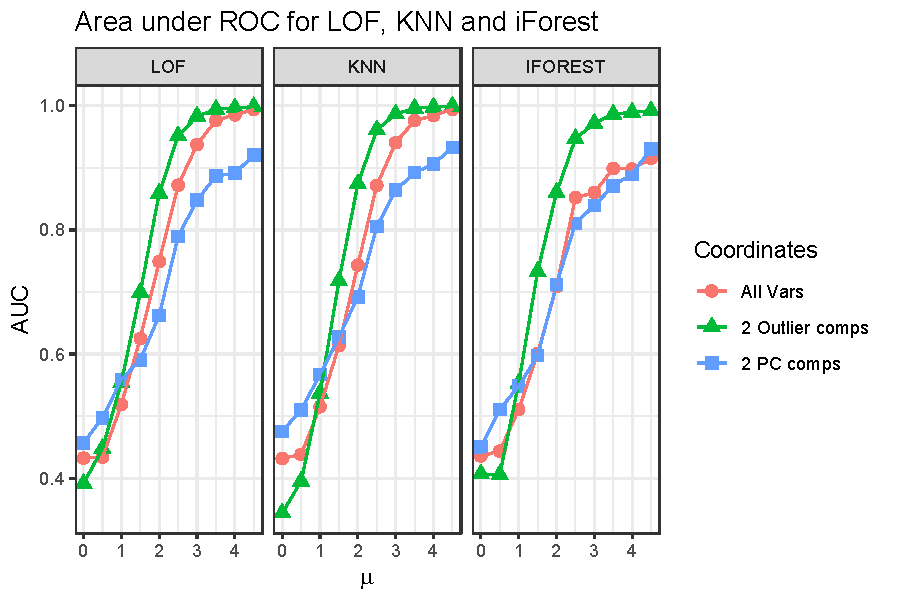
\includegraphics[scale=0.8]{Exp1.pdf}
	\caption{Results of Experiment 1}
	\label{fig:Exp1}
\end{figure} 

Using $2$ outlier components as the coordinates gives the highest performance for all $3$ outlier detection methods for $\mu > 1$.  Indeed, we are interested in a set of coordinates can accentuate the the outliers as they move out from the inlier distribution.  For values of $\mu \in \{0, 0.5, 1\}$,  the outlier distribution lies in the interior of the inlier distribution, making a comparison between the coordinates not meaningful.   

\subsection{Experiment 2}
The second experiment is ***********
% =======================================================================
\section{Results with visualization}
% =======================================================================
FOR LATER!

% =======================================================================
\section{Results on a data repository}
% =======================================================================
FOR LATER!

% =======================================================================
\section{Conclusion}
% =======================================================================
FOR LATER!

% =======================================================================
\footnotesize
\bibliographystyle{agsm} %Choose a bibliograhpic style
\bibliography{Master}
% =======================================================================
\end{document}
